\chapter{Results}

\begin{comment}
In this chapter I will present the results of my analysis.\\
Software:\\
Software engineering:\\
-what issues with the structure of different openMNGlab version did I encounter\\
-What are the needs of different users of the framework in the end?\\

Spike Analysis:\\
-Describe quantifiers and discuss the results of analysing the experimental recordings\\
-image of table containing everything the jupyter notebook has computed\\
-table with info on electrical frequency levels in each recording\\
-diagram showing a quantifier (peak firing frequency) and electrical frequency for each spike train of single recording\\
-compare diagrams of different recordings\\
-compare different quantifiers in one diagram with each other for the same file\\
-compare ISI to log(ISI) for every train in one file\\
\end{comment}


\section{Software}
\subsection{Finished analysis pipeline}
The software development described in the previous chapter resulted in a single jupyter notebook, which represents the current analysis pipeline for this thesis. A schematic version of this pipeline can be seen in figure TODO. The import of the data consists of two separate importing steps. First we use the Neo importer from the current version of our framework to extract the information about the underlying electrical stimulation. After that we use the importer from the old version of openMNGlab to get the rest of the required information. The next part contains some internal processing steps to sort the spike trains and prepare the data for easy representation and quantification in the following steps.\\
Making use of the early versions of OpenMNGlab and the first analysis notebooks from Radomir the event plot for the current file gets computed and visualized. The next step is calculating the inter spike distances, meaning the time between two spikes, and creating inter spike distance graphs for each spike train in the recording.\\
Now follows the main part of quantifier computation. This is where the computations of my chosen quantifiers happens. After all the quantifiers are computed the resulting lists of quantifiers for each spike train get put into a data structure and saved for later reimporting and reuse for further analysis.\\
Now that the quantifiers are calculated it is time to visualize the results. For this, I create different diagrams showing quantifiers over the wholw recording and comparisons of different quantifiers that I will describe in more detail later in this chapter.\\
See the appendix for a detailed view of the whole notebook as well as the code.
%I am not using neo for the spikes because the extraction of mechanical stimuli and corresponding spike trains is connected and already functioning


\section{Spike Analysis}


We have analysed 22 recording files featuring  mechanical and electrical stimulation. An overview for the data can be found in  Table~\ref{table:recording_overview}. Here we see the number of spike trains in each file and the average spikes per train as well as the average spike train duration.

\begin{comment}
\begin{table}[!ht]
\centering
\begin{tabular}{ |c|c|c|c| }
	\hline
	File number & Number of trains  & Avg. spikes per train & Avg. train duration
	1 & 17 & 12.53 & 0.38 \\
	2 & 34 & 16.62 & 0.39 \\
	3 & 37 & 20.03 & 0.40 \\
	4 & 12 & 4.67 & 0.28 \\
	5 & 11 & 9.18 & 0.25 \\
	6 & 22 & 8.55 & 0.12 \\
	7 & 17 & 10.82 & 0.38 \\
	8 & 16 & 7.38 & 0.40 \\
	9 & 28 & 12.93 & 0.37 \\
	10 & 35 & 8.83 & 0.35 \\
	11 & 37 & 15 & 0.41 \\
	12 & 31 & 13.45 & 0.38 \\
	13 & 18 & 10.28 & 0.24 \\
	14 & 22 & 35.64 & 0.44 \\
	15 & 32 & 13.91 & 0.13 \\
	16 & 32 & 25.53 & 0.39 \\
	17 & 33 & 30.45 & 0.23 \\
	18 & 33 & 29.30 & 0.31 \\
	19 & 31 & 11.74 & 0.38 \\
	20 & 48 & 10.85 & 0.40 \\
	21 & 51 & 22.8 & 0.24 \\
	22 & 50 & 12.16 & 0.36\\
	\hline
\end{tabular}
\caption{This table shows a little overview over the available recording files for this thesis.}
\label{table:recording_overview}
\end{table}
\end{comment}

\subsection{Experimental Protocol}
This subsection will explain how the recording files are structured to get a better general understanding of the experiments and analysis.

As explained before, the files I am working with feature electrical and mechanical stimulation. For the mechanical stimulation pressure is applied to the nerve fiber in a sinosoidal shape as can be seen in Figure~\ref{fig:spike_train}. The attributes of this type of stimulation, like amplitude or duration, is constant over the course of single recordings. Electrical stimulation functions as background noise and can be seen as simulating a more stressed fiber. The electrical stimulation is applied as electric impulses with a given frequency. The base frequency of this background stimulation is the same for each of the recordings and lies at $0.1$ Hertz. Each recording features at least one segment of increased frequency, which always follow the same pattern. For a duration the electrical impulse frequency gets increased to either $2.0, 4.0$ or $5.0$ Hertz. After the section of the increased frequency, the frequency first drops to $0.5$ Hertz before going back to$0.1$ Hertz.\\
Each file features at least one burst of increased frequency at one of the mentioned levels. The files in Table~\ref{table:recording_overview} are ordered according to the frequencies of electrical stimulation that occurred in the recordings. Files $1-3, 4-12, 13-14$ contain only frequencies of $2.0, 4.0, 5.0$ Hertz respectively. Files $15-20$ contain both $2.0$ and $4.0$ Hertz frequencies and files $21-22$ contain all three types of increased frequencies.\\

\subsection{Sample Analysis}
Now I will present the results of the analysis notebook with the help of an example. I will take recording 21 from the list of recordings and show the different visual results and quantifiers that were computed.

\subsubsection{Table of values}
When applying the analysis notebook to a single recording one output we get is a big table containing the finished quantifiers as well as the original timestamp values for the spikes. A sample table can be seen in Table~\ref{fig:table_sc}, which shows a screenshot of the output table for file 21. The first 6 rows before the first yellow divider has information about the mechanical stimulus such as amplitude, duration and time to the next stimulus event. The next section between the two yellow dividers shows single value quantifiers such as peak firing frequency and mean firing rate for each spike train. The third section below the second yellow divider contains lists of raw values that were used to compute the single value quantifiers.\\
\begin{figure}
	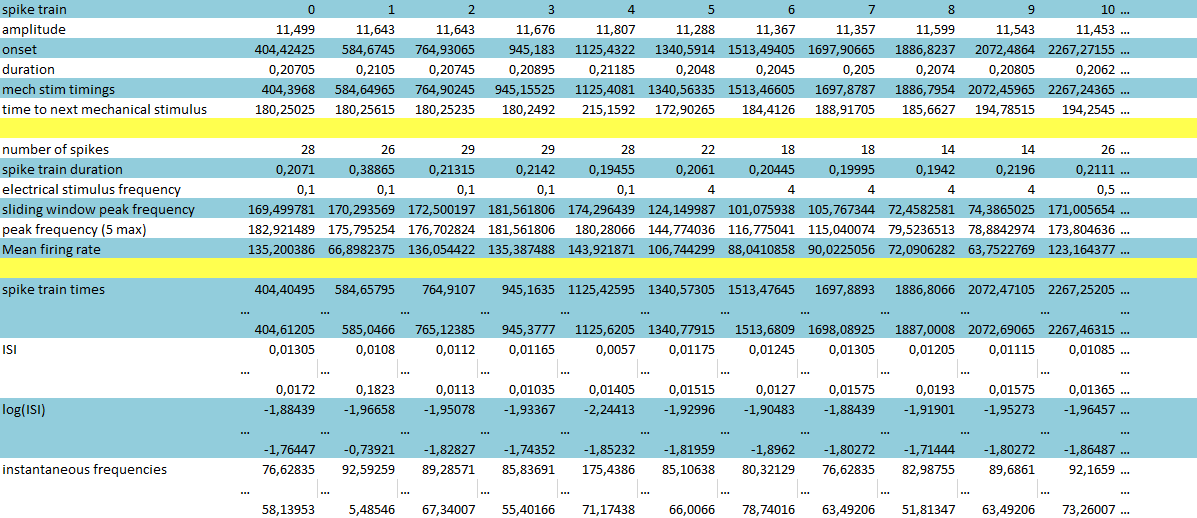
\includegraphics[width = \textwidth]{src/pic/sc_table}
	\caption{Sample picture of table after successful analysis }
	\label{fig:table_sc}
\end{figure}

\subsubsection{Event plot}
A figure that we have seen previously in this thesis is the event plot \ref{fig:eventplot}. It shows an overview of spiking activity after mechanical stimuli over the course of a whole recording. It is not meant to be an in depth analysis tool, but rather a quick visual representation of a recording.

\subsubsection{Comparative diagrams for quantifiers}
\begin{figure}
	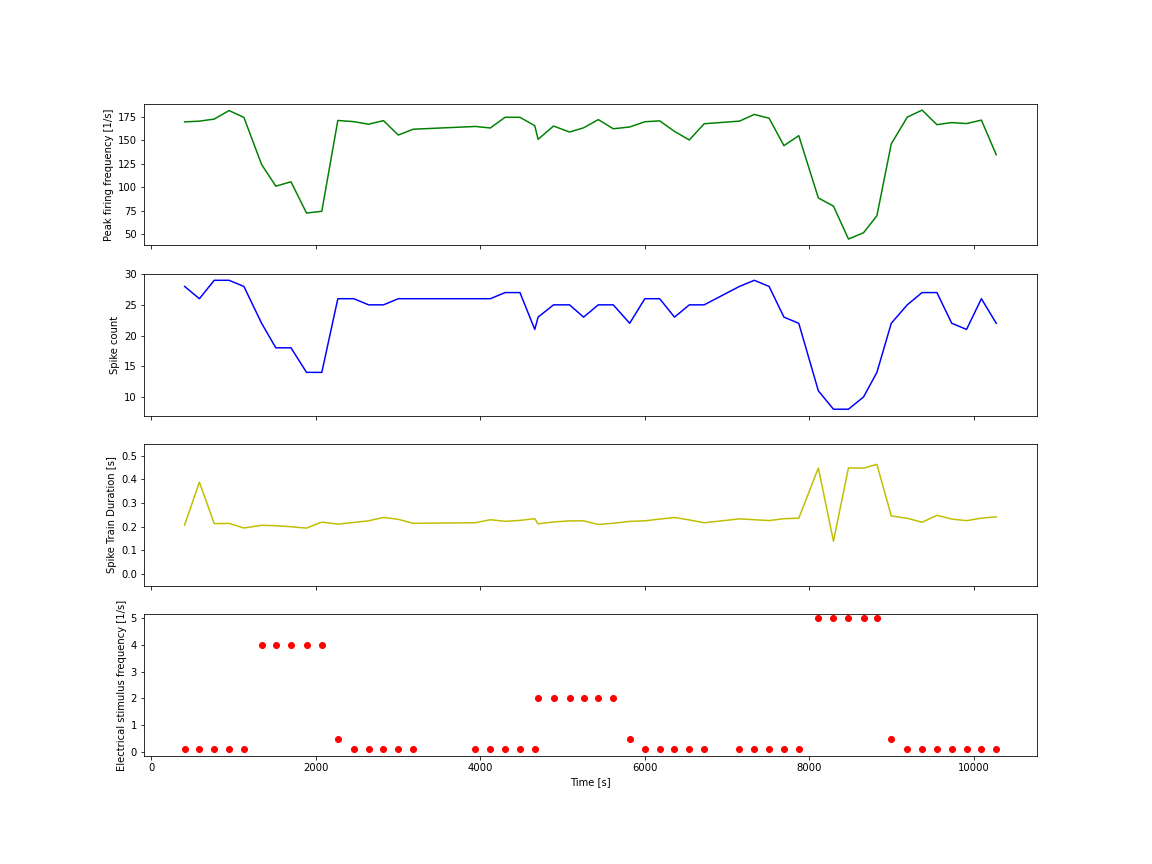
\includegraphics[width = \textwidth]{src/pic/11_12_13_sp}
	\caption{Diagram showing a separated comparison of peak firing frequency and spike count for recording 21}
	\label{fig:quantcomp_sp}
\end{figure}
\begin{figure}
	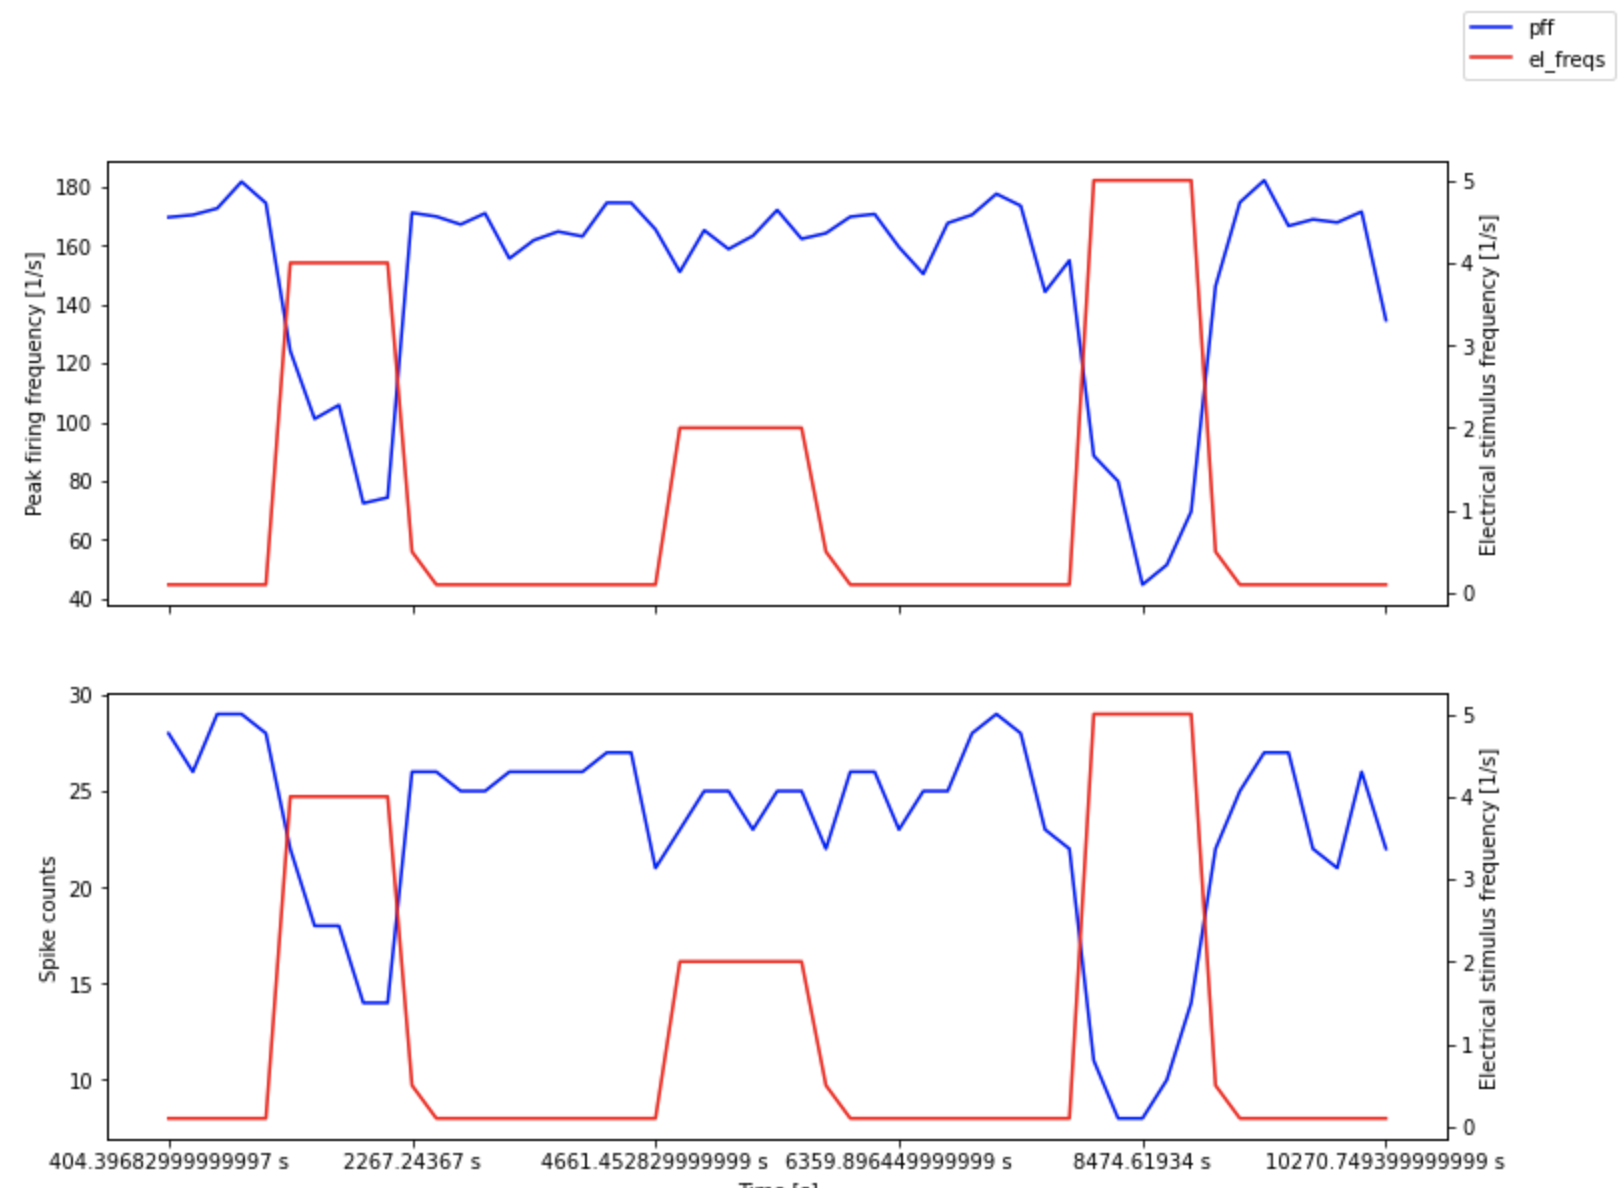
\includegraphics[width = \textwidth]{src/pic/11_12_13_cm}
	\caption{Diagram showing a comparison of peak firing frequency and number of spikes for recording 21}
	\label{fig:quantcomp_cm}
\end{figure}


%selected additional information in more detail:

%-diagram of peak firing frequency, spike counts, train duration and electrical frequency\\
%-shows the correlation between electrical frequency and the other quantifiers of single spike trains\\

%-diagrams of Interspike Intervals(isi) and logarithm of isi\\
%-should show that by taking the logarithm, the isi becomes more linear\\




\cleardoublepage
